\chapter{Background}

In Machine Learning, Hyperparameter Optimization or “Tuning” is the process of choosing the optimal Hyperparameters for the learning algorithm \cite{Tesi-1.10}.
Where an “Hyperparameter” is a value used to control the learning process, basically a parameter of the Learning Algorithm and not of the model itself \cite{Tesi-1.6}.
\\[0.3cm]Thus, Hyperparameter Optimization has the goal to determine the best tuple of Hyperparameters which can minimize the value of the Loss Function \cite{Tesi-1.1}.
The process of selecting the right Hyperparameters configuration is called “Hyperparameter Optimization” or “Hyperparameter Tuning”.


\section{Introduction to Hyperparameter Optimization}

\myparagraph{Reason for Tuning Hyperparameters:}
The Hyperparameters allow Machine Leaning models to be customized, or tuned, for specific tasks or dataset \cite{Tesi-1.6}.
Basically, one important aspect of Hyperparameters is to allow a particular model to be reused in different situations and different datasets.
\\[0.3cm]Generally, what each Hyperparameter does when considered alone is known; but it is hard to predict what the best combination of Hyperparameters is the best for a specific problem or specific dataset.


\myparagraph{Necessity and Importance of Hyperparameter Optimization:}
Hyperparameter Optimization is generated from the necessity to automate the boring and expensive process of manually setting via trial-and-error the Hyperparameters of Machine Learning models \cite{Tesi-1.6}.
Choosing the optimal architecture for the model is not an easy task, and in many cases the possibilities are so many it is impossible for a human to select the best possible configuration.
Thus, the ideal solution would be to make the machine to learn the optimal configuration by itself, exploring different model architectures to find the better performing one.
Without automated Hyperparameter Optimization the programmer can only rely on trial-and-error and empirical experience.
\\[0.3cm]Hyperparameter Optimization (HPO) algorithms have not only to automate the process of researching for the best Hyperparameters combination, but also to make this search computationally viable even for more complex models and problems.
The main challenge of Hyperparameter Optimization is that is hard to predict how the Hyperparameters could influence each other's. This uncertainty makes the problem even more complex computationally, as pratically all possibilities must be explored. 

\subsection{Introduction}

Machine Learning is about predicting and classifying data. ML Models do so using parameters, meaning that the Models are Parametrized so that their behaviour is tuned for any given problem.
The large term “Parameter” in Machine Learning can divide in two categories: Parameter (or Model Parameter) and Hyperparameter.

\subsubsection{Parameters}

A model Parameter is a configuration variable internal to the model.
The Parameters are part of the model, are learned by training from data, they define the skill of the model and are thus required to make predictions.
The Parameters in Machine Learning models have the same function that variables have in traditional programming.
\\[0.3cm]Examples of Parameters in various Machine Learning models: Weights (in Neural Networks); Support Vectors (in SVM); Coefficients (in Linear or Logistic Regression).

\subsubsection{Hyperparameters}

A model Hyperparameters is a configuration that is external to the model.
The Hyperparameters cannot be learned from the data and are often set by the programmer. Their values are either determined by heuristics or by optimization techniques.
\\[0.3cm]Basically, Hyperparameters are not Parameters of the Model itself, but are rather Parameters of the leaning process/algorithm used to train the model.
\\[0.3cm]Examples of Hyperparameters in various Machine Learning models: Learning Rate and Epochs (in Neural Networks); $C$ and $\delta$ (in SVM); $k$ (in k-nearest neighbors).

\subsection{Basic Concepts of Hyperparameter Optimization}

Two fundamental concepts of Hyperparameter Optimization, indispensable in the understanding of HPO, are Objective Function and Search Space.

\subsubsection{Objective Function}

An Objective Function, in Optimization problems, is the opposite of a Loss Function. More precisely, is a “scoring function”, it serves as a metric to define the performance of the trained model \cite{Tesi-1.1} \cite{Tesi-1.6}.
\\[0.3cm]The performance of a learning algorithm can be seen a function:  $f: X \to \mathbb{R}$, that maps the Hyperparameters space $X \in \textbf{X}$ to the result of the Validation function.
Basically $f(X)$ represents an evaluation of the model trained with the tuple $X$ of Hyperparameters.
\\[0.3cm]The goal of Hyperparameter Optimization is to Minimize or Maximize (depends on the Evaluation metric) the value of $f$, particularly, the tuple $X$ of Hyperparameters that permits so.

\subsubsection{Search Space}

In order to search for the best combination of Hyperparameters, a Search Space has to be defined.
The Search Space, or Configuration Space, denoted with $\textbf{X}$, is the multidimensional table of all the possible values the Hyperparameters can be \cite{Tesi-1.6}.
\\[0.3cm]A Seach Space is a Multidimensional object, where each dimension represents a Hyperparameter, and each point represents a particular Hyperparameters configuration.
More specifically, each point in the Search Space is vector, or tuple, containing the values for each Hyperparameter of that combination.

\subsection{Fundamentals Components of a HPO Algorithm}

In general, all complex HPO algorithms two principal components: Samplers and Pruners (also called Searching and Scheduling).
\\[0.3cm]The Sampler, or Search Algorithm, decides which configuration to try.
The Pruner, or Scheduler, decides how to allocate the computational budget and when to stop a trial.
\\[0.3cm]On top of these two components, it is to be considered the Tuner, the class that executes the optimization process. Reaching the total three main components.
\\[0.3cm]The concept of a class (the Tuner) which abstracts and executes the Optimization Process, and the concept of Searchers (Sampler) and Schedulers (Pruner) are widely applied in many Hyperparameter Optimization libraries.

\subsubsection{Sampler}

A Sampler, or Searcher, in HPO is the component of the HPO algorithm which selects (“samples”) the next candidate configurations to try and evaluate.
Simple Samplers like Grid Sampler (for Grid Search) and Random Sampler (for Random Search) just select candidates sequentially and randomly respectively; more complex Samplers, used for example in Bayesian Optimization, make the decision based on previous trials.
\\[0.3cm]In the making of the choice of the Sampler, it is important to understand that Hyperparameters not always have the same importance in the results of the model. Also, some Samplers are more effective with certain models than others. (See Fig.~\ref{fig:figure-2.1.1})
\begin{figure}[t]
	\centering
	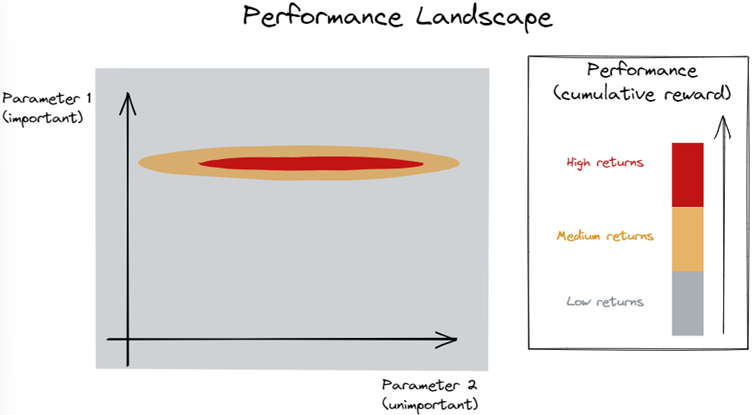
\includegraphics[width=11cm]{figures/figure-2.1.1.png}
	\caption[Hyperparameters Importance]{A Graph showing how the importance of Hyperparameters can be spread in the Search Space. Source:~\cite{Tesi-1.3}}
	\label{fig:figure-2.1.1}
\end{figure}

\subsubsection{Pruner}

A Pruner, or Scheduler, in HPO is the component of the HPO algorithm which determines if and when a trial needs to be stopped in order to dedicate more resources to more promising candidates.
The Pruner has the goal to identify and then discard the bad performing configurations.
The final objective is to ensure more computational resources to the remaining configurations.
\\[0.3cm]It is important to understand when to prune. If pruning too early, the selection would be too premature, and some potentially good configuration may be discarded. If pruning too late, resource would have been wasted on bad configurations.
\\[0.3cm]The most basic Pruners, on which more complex Pruners are based, are Median Pruner and Successive Halving.
The Median Pruner is the simplest Scheduler (Pruner). At each step, all the configuration with a worse performance than the median of the results in that step, gets discarded. (Fig.~\ref{fig:figure-2.1.2})
\begin{figure}[t]
	\centering
	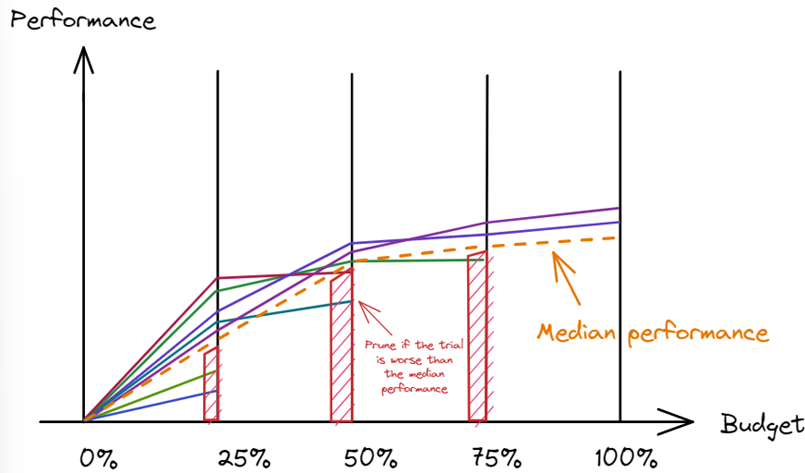
\includegraphics[width=12cm]{figures/figure-2.1.2.png}
	\caption[Pruning Algorithm]{A Graph showing the generic functioning of a Pruner Algorithm; in this case, a Median Pruner is showed. Source:~\cite{Tesi-1.3}}
	\label{fig:figure-2.1.2}
\end{figure}
\\[0.3cm]Successive Halving is a slightly more complex Pruning algorithm than Median Pruner. The idea is simple: it starts with some configurations, at some point they get pruned, and only the most promising ones remain. The complex part is that this whole process is determined by Hyperparameters. Which are: the minimum budget, the initial number of trials, and the percentage of configurations to discard at each step.
\\More of Successive Halving Algorithm and Pruning algorithms in general will be discussed in the following sections.

\subsubsection{Tuner}

The Tuner, in HPO is the function that wraps up the Optimization Process. The Tuner runs the Sampler and the Pruner, manages the optimization of the process (like parallelizing), records the results and the possible errors of each trial.
The Tuner can keep records of various information of the Optimization Process, such as errors, runtime, index of the configuration, suggestions of the Samplers, pruning actions of the Pruner.

\section{Hyperparameter Optimization Algorithms}

The goal of a Hyperparameter Optimization Strategy is to find the configuration of Hyperparameters, which lead, after the training of the model, to the minimum error and the maximum performance.
There are many Hyperparameter Optimization techniques, some are specialized for specific ML models, other are more generic.
\\[0.3cm]The HPO algorithms can be divided into 2 main categories: Black-Box Optimization algorithms, and Multi-Fidelity HPO algorithms (Fig.~\ref{fig:figure-2.2.1}).
The first category is manly based to the use of Samplers, the second category uses Early Stopping and Pruners.
\begin{figure}[t]
	\centering
	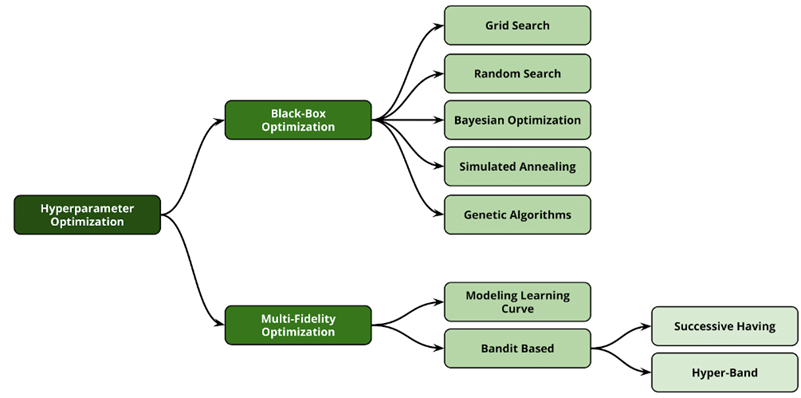
\includegraphics[width=15cm]{figures/figure-2.2.1.png}
	\caption[Hyperparameter Optimization Algorithms]{Categories of Hyperparameter Optimization Algorithms. Source:~\cite{AutomatedML}}
	\label{fig:figure-2.2.1}
\end{figure}

\subsection{Grid Search}

Grid Search is a traditional way to perform Hyperparameter Optimization. It simply consists of an “Exhaustive Search” of the Optimal Hyperparameters between a subset of specified Hyperparameters.
\\[0.3cm]Grid Search is an approach that will methodically build and evaluate the model for each possible combination of Hyperparameters' values (Fig.~\ref{fig:figure-2.2.2}).
\\[0.3cm]The performance of a determined configuration of the Hyperparameters for the training of the model is evaluated using techniques such as Cross-Validation or Hold-One-Out.
This evaluation is done for each tuple of Hyperparameters. At the end, the configuration with the best performance is the optimal set of Hyperparameters for that model.
\begin{figure}[t]
	\centering
	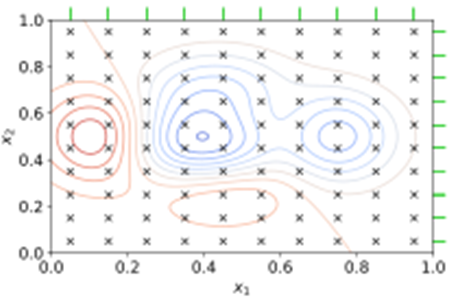
\includegraphics[width=8cm]{figures/figure-2.2.2.png}
	\caption[Candidates Distribution in Grid Search]{Distribution of Candidate Configurations over the Search Space in Grid Search. Source:~\cite{Tesi-1.1}}
	\label{fig:figure-2.2.2}
\end{figure}

\myparagraph{Application of Grid Search:}
For each Hyperparameter, the programmer defines the range of values that each Hyperparameter can be. Each of these lists of values can be seen as an Array of values, each referring to a Hyperparameter.
The whole of these Arrays will then form a Grid. In the Grid Search technique, the Cartesian Product is applied to obtain all the possible combinations of values \cite{Tesi-1.2}.
The outputs are the setting (the configuration of Hyperparameter) which achieved the highest score, the best performance.

\myparagraph{Advantages and Disadvantages of Grid Search:}
The main Pro of Grid Search is that is an “Embarrassingly Parallel” problem, which means that it is very easy to parallelize the operations.
The big Con, on the other hand, is that this technique suffers from the “Curse of Dimensionality”, its complexity tends to escalate exponentially very easily, given that there is a Cartesian Product involved \cite{Tesi-1.10}.
\\[0.3cm]Also Grid Search can suffer from “Unlucky Search”, where none of the possible combinations obtained from the Param Grid obtains high results. (Fig.~\ref{fig:figure-2.2.3})
\begin{figure}[t]
	\centering
	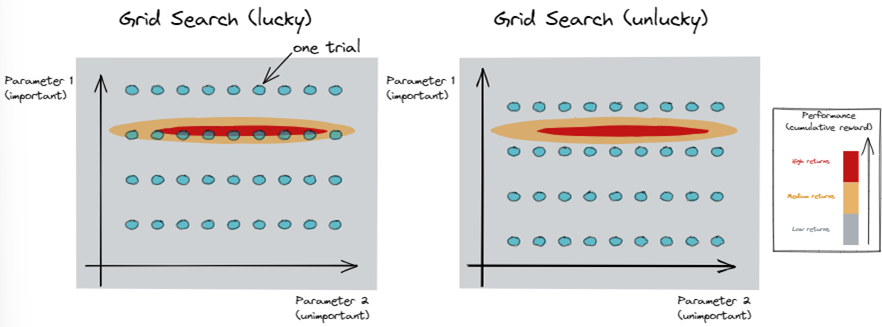
\includegraphics[width=15cm]{figures/figure-2.2.3.png}
	\caption[Unlucky Search]{Graph comparison showing the phenomenon of “Unlucky Seach” in Grid Search. Source:~\cite{Tesi-1.3}}
	\label{fig:figure-2.2.3}
\end{figure}

\subsection{Random Search}

Random Search is an alternative Hyperparameter Optimization technique to Grid Search \cite{OptunaSamplers-RandomSearch}.
It replaces the “Exhaustive Enumeration” of all possible Hyperparameter combinations with a simple Random Selection of these combinations (Fig.~\ref{fig:figure-2.2.4}).
\\[0.3cm]Random Search is an approach where rather than defining determined values for the Hyperparameters, statistical distributions are defined, which are used to randomly select values from them.
\\[0.3cm]Differently from Grid Search, is able to explore much more values for both discrete and continuous Hyperparameters; it is an “Explorative” technique.
It is considered an important baseline for comparing the performance of the newer Hyperparameters Optimization techniques.
\begin{figure}[t]
	\centering
	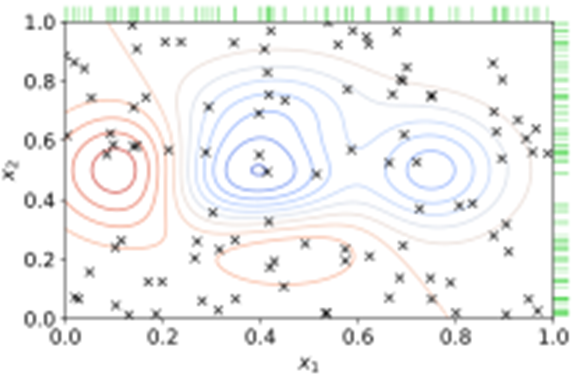
\includegraphics[width=8cm]{figures/figure-2.2.4.png}
	\caption[Candidates Distribution in Random Search]{Distribution of Candidate Configurations over the Search Space in Random Search. Source:~\cite{Tesi-1.1}}
	\label{fig:figure-2.2.4}
\end{figure}	

\myparagraph{Advantages of Random Search:}
Random Search can outperform Grid Search, especially when the number of Hyperparameter which heavily effects the learning process is small \cite{OptunaSamplers-RandomSearch}.
As Grid Search, Random Search is also an Embarrassingly Parallel problem.
\\[0.3cm]Despite these advantages, Random Search is still very basic, and it is not rigorous.

\myparagraph{Comparing Grid Search and Random Search:}
Random Search can resolve the “Unlucky Search” problem of Grid Search (Fig.~\ref{fig:figure-2.2.5}).
Random Search is also better performing to the “Curse of Dimensionality”, that is, when there are many dimensions involved.
\\[0.3cm]The advantage of Random Search lies in the fact that Hyperparameters, most of the time, are not equally important, and so strategies that examine all the possibilities, are most of the times losing time on useless evaluations \cite{Tesi-1.2}.
\begin{figure}[t]
	\centering
	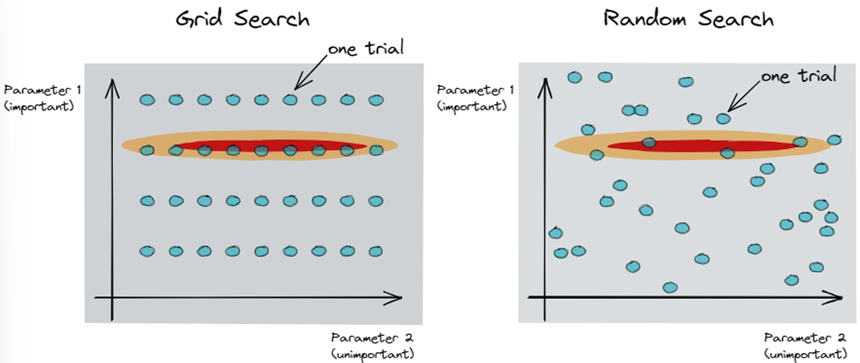
\includegraphics[width=15cm]{figures/figure-2.2.5.png}
	\caption[Grid Search and Random Search Comparison]{Graph comparison between the distribution of candidate configurations in Grid Search and Random Search. Source:~\cite{Tesi-1.3}}
	\label{fig:figure-2.2.5}
\end{figure}

\myparagraph{Choosing between Grid Search and Random Search:}
Grid Search and Random Search are the simplest Hyperparameters Optimization techniques, so are utilized when the problem is fairly simple and does not involve extreme complexity.
Also, both Grid and Random Search tend to become very expensive when the complexity grows, Grid Search especially \cite{Tesi-1.4}.
\\[0.3cm]In general, Grid Search is more appropriate for problems where the most common best values for a Hyperparameter are already known, and so the search is about finding the best combination between those already good-performing values.
\\[0.3cm]Random Search on the other hand, is more appropriate for discovering new Hyperparameters values or new unexpectedly good combinations.

\subsection{Bayesian Optimization}

Bayesian Optimization is a Hyperparameter Optimization technique which builds a probabilistic model of the target function mapping the Hyperparameters values to the performance obtained on the Validation Set \cite{OptunaSamplers-TreeStructuredParzenEstimator}.
\\[0.3cm]Basically, this methos smartly explores the potential optimal configurations of the Hyperparameters' values, basing its decision on the performance of the previous configuration. (Fig.~\ref{fig:figure-2.2.6})
\begin{figure}[t]
	\centering
	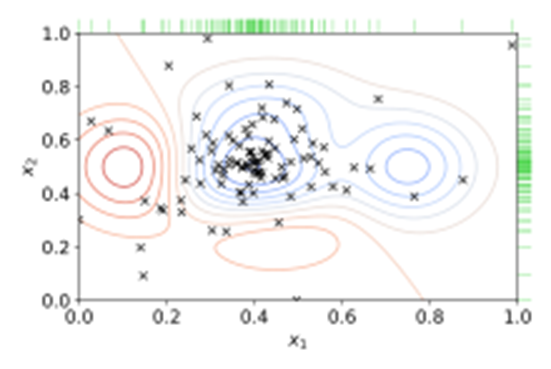
\includegraphics[width=8cm]{figures/figure-2.2.6.png}
	\caption[Candidates Distribution in Bayesian Optimization]{Distribution of Candidate Configurations over the Search Space in Bayesian Optimization. Source:~\cite{Tesi-1.1}}
	\label{fig:figure-2.2.6}
\end{figure}

\myparagraph{Exploitation vs Exploration:}
In HPO, an important trade-off is the one between Exploitation vs Exploration.
Exploitation is the concept of exploiting, using, those value which are already expected to be closed to the optimum.
Exploration is the concept of trying new unexplored risky values which could improve the performance and add new knowledge about a particular Hyperparameter.
\\[0.3cm]Bayesian Optimization balances Exploitation and Exploration, considering both concept in order to get closer to the Optimum.

\myparagraph{Application of Bayesian Optimization:}
The main idea of Bayesian Optimization is to estimate the performance of a certain configuration before that configuration gets tried.
The Bayesian Optimization starts randomly from one configuration, or from a configuration which is already known to be at least decent.
Then a probabilistic model (Acquisition Function) of the Objective Function is built, the idea is to predict which configuration will maximize the value of the performance, the found configuration will be the next.
At each iteration the Acquisition Function is updated, and thus, the prediction becomes more and more accurate.
Bayesian Optimization can find the best Hyperparameter Configuration much faster than traditional search algorithms.

\subsection{Gradient-based Optimization}

Gradient-Based Optimization is a Hyperparameter Optimization technique used with specific Machine Learning model such as Neural Networks and SVMs \cite{Tesi-1.8} \cite{Tesi-1.1}. 
\\[0.3cm]The Hyperparameters are optimized just like the model Parameters, with Gradient Descent.
The more traditional approach of this optimization algorithm uses “Automatic Differentiation” to calculate the so called “Hypergradients”, to update the values of Hyperparameters. Basically, the Gradient of the model is also used during HPO.
\\[0.3cm]While using this method would actually be more efficient, it requires to calculate second-order derivates, which are computationally expensive to approximate. These techniques are therefore very rarely used, because are difficult to apply.
\\[0.3cm]More recent and complex techniques are now being developed for the Gradient-Based Optimization, making it more efficient and able to work with Discrete Hyperparameters.

\subsection{Evolutionary Optimization}

Evolutionary Optimization is a Hyperparameter Optimization technique which follows a process inspired by biological concept of Evolution.
Evolutionary Optimization is applied in almost all fields of Machine Learning, from Statistical ML to Neural Networks and especially in Deep Learning \cite{Tesi-1.1} \cite{OptunaSamplers-NSGAII} \cite{OptunaSamplers-CMA-ES}.

\myparagraph{Steps of Evolutionary Optimization:}
Evolutionary Optimization consists in a series of steps, each of which is inspired by a step of the Theory of Evolution.
\begin{enumerate}[itemsep=0.1cm]
    \item Create an initial population of random solutions (random Hyperparameters values configurations)
    \item Evaluate the Hyperparameters tuples (configurations) and obtain their “Fitness Function” (a particular type of Objective Function that summarizes the results of each score metric)
    \item Rank the Hyperparameters tuples by their Fitness Function value.
    \item Replace the worst tuples with new tuples generated through crossover and mutation (where Crossover and Mutation are the same concepts as they are in Biology)
    \item Go back to step 2 until the performance goal of the algorithm is reached or until the performance is no longer improving.
\end{enumerate}

\subsection{Population-based Training}

Population-Based Training (PBT) is a Hyperparameter Optimization algorithms family; it is a broader optimization technique, applied to learn both Hyperparameters values and network weights (or model's parameters in general).
\\[0.3cm]Population-Based Training is very similar to Evolutionary Optimization, actually the latter is a particular case of Population-Based Training.
\\[0.3cm]PBT is very flexible and can be applied to a wide range of different models or problem domains. The optimization process does not depend on aspects like Network Architecture, particular Loss Function, etc.

\myparagraph{Main Difference with Evolutionary Optimization:}
Like Evolutionary Optimization, Population-Based Training (PBT) involves iteratively replacing poorly performing configuration with better performing modified.
\\[0.3cm]The first difference between PBT and Evolutionary Optimization is that in PBT are not necessarily used Evolutionary Algorithms, but rather a wider range of techniques are applied.
Another main difference is the fact that configurations at each generation are not replaced, but rather updated.
\\[0.3cm]In PBT, when possible, the concept of “Warm Starting” is often used, where models are initialized with hyperparameters and weights from already known better configurations to speed-up the training process \cite{Tesi-1.1}.

\subsection{Early Stopping-based Techniques}

Early Stopping-Based Training is a Hyperparameter Optimization technique family, or rather, are techniques that are often used in combination with the other approaches in order to improve the efficiency of the optimization process.
\\[0.3cm]These techniques are mainly applied for models that have a large number of Hyperparameters and a large number of possible values for those.
\\[0.3cm]The main idea of Early Stopping-Based Training is to iterate between some configurations in searching of the most promising one, using statistical tests to discard bad configurations \cite{Tesi-1.3}.

\myparagraph{Early Stopping-Based Algorithms:}
\newline Successive Halving Algorithms (SHA) begins as a random search of the optimal configuration, and periodically halves the trials, removing the worst-performing ones.
\newline Asynchronous Successive Halving Algorithms (ASHA) improves the performance of SHA, executing the process asynchronously.
\newline Hyperband invokes SHA or ASHA multiple times, with different levels of “aggressiveness”.
\newline Bayesian Optimization and Hyperband (BOHB) is a combination of Bayesian Optimization and Hyperband.
\\[0.3cm]These and other Early Stopping-Based Algorithms will be discussed in the following section regarding Multi-Fidelity Hyperparameter Optimization.

\section{Multi-Fidelity Hyperparameter Optimization}

Hyperparameter Optimization is one of the most computationally expensive processes in the Training of a Machine Learning model.
At the start of Hyperparameter Optimization, a number n of configurations to try is chosen. The ideal solution of course is to try every single configuration, to be sure to find the best one.
But when the model is to complex, the budget, intended as computational budget, is limited, and try every single configuration fully is not the most efficient strategy.
The solution is to use Multi-Fidelity Hyperparameter Optimization.

\myparagraph{Optimizing the Tuning Process:}
The main idea is to early-stop a trial of a particular configuration if that trial is not promising.
At the start of the search, each configuration is given the same (low) amount of computational budget. At one point, the least promising configurations up to that point are abandoned, and the remaining are given more budget.
\\[0.3cm]This process gets iterated, until at the last iteration only a small set of configurations will have the whole budget to complete their evaluation. (Fig.~\ref{fig:figure-2.3.1})
\begin{figure}[t]
	\centering
	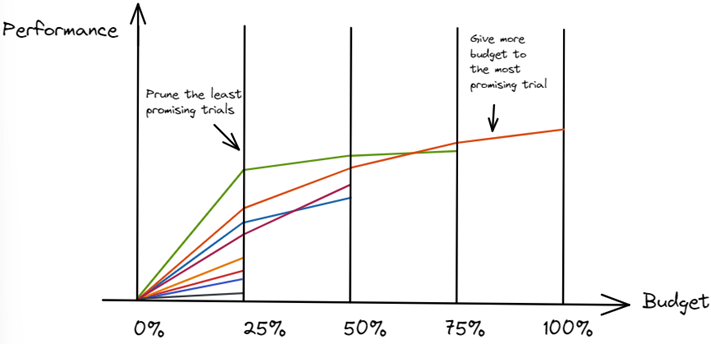
\includegraphics[width=14cm]{figures/figure-2.3.1.png}
	\caption[Multi-Fidelity HPO Process Example]{Graph showing an example of an Multi-Fidelity HPO; this particular example could represent different types of Pruners as Median, SHA or Hyperband. Source:~\cite{Tesi-1.3}}
	\label{fig:figure-2.3.1}
\end{figure}

\subsection{Introduction to Multi-Fidelity HPO}

When applying for Hyperparameter Optimization algorithms on Neural Networks, the workload is much bigger than any other Machine Learning model.
Using parallelization techniques enables to reduce the time of the processes, but the workload itself still remains the same.
\\[0.3cm]With Multi-Fidelity Hyperparameter Optimization, is possible to reduce the total computational workload the machine has to go through during the Optimization Process.
Multi-Fidelity HPO uses Early Stopping and Pruners. Pruners determine if and when an unpromising trial needs to be stopped early, pruned.

\myparagraph{Process of Multi-Fidelity HPO:}
After a few epochs of the trial of one Hyperparameters Configuration, it is already visually evident if that trial is or not promising.
The Pruner algorithm decides when and how to stop those unpromising trials, allowing only the promising trials to complete the number of epochs and thus fully complete the training.
\\[0.3cm]During each “Rung” (“Step”) of the process, each trial is partially evaluated using the Validation Error, the Validation Error (or any other metric, evaluated on the Validation Set) is used as an estimate of the final score of the configuration.
Which precise value the trial should reach to proceed to the next Rung, depends on the Pruning algorithm.

\subsection{Multi-Fidelity HPO Algorithms}

Multi-Fidelity HPO algorithms divides in Multi-Armed Bandit approaches, and Modeling Learning Curve approaches. The most important ones are the Multi-Armed Bandit (MAB) approaches. (Fig.~\ref{fig:figure-2.3.2})
\begin{figure}[t]
	\centering
	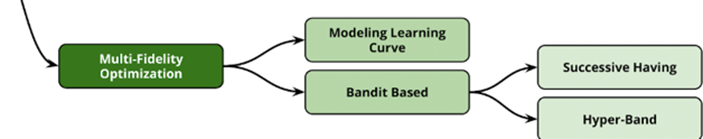
\includegraphics[width=15cm]{figures/figure-2.3.2.png}
	\caption[Multi-Fidelity Hyperparameter Optimization Algorithms]{Categories of Multi-Fidelity Hyperparameter Optimization Algorithms. Source:~\cite{AutomatedML}}
	\label{fig:figure-2.3.2}
\end{figure}
\\[0.3cm]The main characteristics of MAB algorithms are the Dynamic allocation of resources, and the balance between Exploration and Exploitation.
\\[0.3cm]The most important MAB algorithms are: Successive Halving (SHA), Hyperband, Iterated Racing, ASHA, BOHB.
The most basic Multi-Fidelity HPO MAB algorithm is Successive Halving (SHA). All the basic aspects of SHA, like the trade-off between trials and budget, are valid for all MAB algorithms.

\subsubsection{Successive Halving}

Successive Halving can be seen as a tournament among the candidates (Hyperparameter Configurations) of the HPO process.
The Successive Halving algorithm divides the “searching” process in iterations, that are often called “Rungs”. At the end of each Rung level, only the best (most promising) candidates pass to the next level \cite{Tesi-1.7} \cite{OptunaPruners-SuccessiveHalvingAlgorithm}. (Fig.~\ref{fig:figure-2.3.3})
\begin{figure}[t]
	\centering
	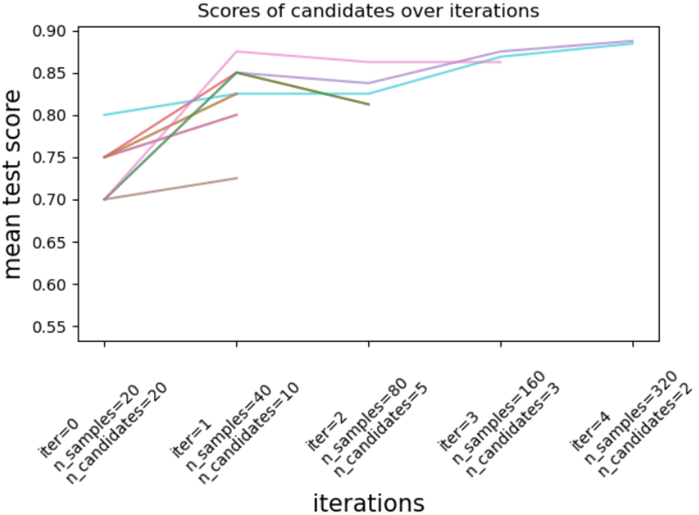
\includegraphics[width=11cm]{figures/figure-2.3.3.png}
	\caption[Successive Halving Algorithm Example]{Graph showing an example of an Optimization using Successive Halving Algorithm. Source:~\cite{Tesi-1.7}}
	\label{fig:figure-2.3.3}
\end{figure}

\myparagraph{Number of Candidates and Amount of Resources:}
The two most important aspects of Successive Halving are the Number of Candidates and the Amount of Resources dedicated at each iteration.
Each Rung has a number of Candidates and an Amount of Resources; the rule which determines how and how much those quantities should vary at each Rung depends on the Pruning algorithm.
In simpler Pruning algorithms like Successive Halving, the parameter which control how much the two quantities should vary is called Factor \cite{OptunaPruners-SuccessiveHalvingAlgorithm}.

\myparagraph{Factor:}
In simpler Pruning algorithms like Successive Halving, the parameter which control how much the two quantities should vary is called Factor.
\\[0.3cm]Factor controls the rate at which the resources grow and the number of candidates decreases.
At each Rung, the number of resources (per candidate) is multiplied by Factor, and the number of candidates is divided by Factor \cite{OptunaPruners-SuccessiveHalvingAlgorithm}.

\myparagraph{Resource:}
The resource parameter is the particular data or metadata to use as “budget”.
The choice of this “Resource” depends on the Machine Learning model object of the HPO.
\\[0.3cm]For a model like RandomForest, a good resource is “n\_samples”, which is the fraction of the Dataset on which to train the model.
\\[0.3cm]For Neural Networks the most used data a resource is the Hyperparameter “epochs”. Basically, during successive halving, only the most promising configuration have the opportunity to complete progressively more epochs \cite{OptunaPruners-SuccessiveHalvingAlgorithm}.

\myparagraph{Min\_Resources:}
The parameter min\_resources is the amount of resources allocated at the iteration (per candidate).
This is a very important number for the success of the algorithm, as if it is too small, potentially good candidates may have a bad start and get pruned prematurely; if it is too big, the algorithm will be inefficient, as most candidates, even the worst ones, will consume a lot of resources at the first iterations \cite{OptunaPruners-SuccessiveHalvingAlgorithm}.

\subsubsection{Hyperband}

Hyperband is an HPO algorithm, it is a form of Multi-Fidelity algorithm \cite{OptunaPruners-Hyperband} \cite{Tesi-1.8}.
The idea of Hyperband is to efficiently allocate resources to the Optimization Process, combining Random Searching, Successive Halving, and Early Stopping techniques.
\\[0.3cm]Hyperband work is especially utilized in settings where the amount of available computational resources is limited.
\\[0.3cm]Starting from the total set of Hyperparameters Configuration, Early Stopping and Successive Halving are applied during the training process in order to maintain only the best promising configurations.
At each iteration the amount of resources assigned to each trial is enlarged, allocating thus more resources to best promising configurations.
\\[0.3cm]Hyperband outperforms most traditional HPO algorithms, it is usable for many ML models, it is scalable and parallelizable; it is particularly used in Deep Learning.
Most modern studies are trying to combine Hyperband with Bayesian Optimization, to obtain an even more powerful HPO algorithm.

\subsubsection{Iterated Racing}

Iterated Racing is a complex HPO algorithm based on efficient computational resources allocation to promising configurations \cite{Tesi-1.8}.
\\[0.3cm]The idea of Iterated Racing is to iteratively race configurations against each other, in pair, and then allocate more computational resources to the winning ones, discarding the losing.
The configurations basically participate in a sort of tournament, which ends when a single configuration is remaining or other termination criteria are met.

\subsubsection{ASHA and BOHB}

Asynchronous Successive Halving Algorithm (ASHA) is the Asynchronous version of SHA \cite{OptunaPruners-AsynchronousSuccessiveHalvingAlgorithm}. Trials are executed asynchronously, gaining in efficiency, but increasing the risk of undeservedly promoting bad configurations to the next Rung.
\\[0.3cm]Bayesian Optimization and Hyperband (BOHB) is an extremely complex HPO algorithm, which mixes ASHA, Hyperband and Bayesian Optimization \cite{Tesi-1.10} \cite{Tesi-1.9} \cite{AutomatedML}.
Basically, BOHB is a combination of all the best performing HPO algorithms. It is probably, at least results-wise, the best HPO algorithm at the state-of-the-art.

\section{Hyperparameter Optimization In-Depth}

Hyperparameter Optimization is an expensive procedure, both computationally and effort-wise, so good approaches need to be used to make it more feasible.
\\[0.3cm]Techniques like Parallelization makes the HPO algorithm more efficient.
Overfitting mitigation techniques prevents the HPs to overfit the validation set.
Good practices of HPO coming from Practical Aspects, allow the ML programmer to reduce the time of Trial-and-Error during the set of the algorithm.

\subsection{Parallelization in HPO}

Even when using complex HPO algorithms, the process can take hours or days to finish depending on how big the dataset is, how complex the model to train is, and how many Hyperparameters and Hyperparameter's values are there.
\\[0.3cm]The waiting time could be massively reduced by distributing the trials across parallel resources. There can be distinguish three different types of scheduling: Sequential, Synchronous and Asynchronous \cite{Tesi-1.6}.

\myparagraph{Parallelization in Standard HPO:}
In Sequential HPO there is no parallelization, each trial is executed only after the previous trial.
\\[0.3cm]In Synchronous HPO, the new batch of configurations (set of trials) is sampled when the previous set finishes. This means that if a batch requires more time to finish, the next batch will have to wait for the resource to be released.
\\[0.3cm]In Asynchronous HPO, each new Hyperparameters Configuration is evaluated immediately after the previous one is finished; so, each parallel worker is always busy \cite{Tesi-1.6}.
\newline (Fig.~\ref{fig:figure-2.4.1})
\begin{figure}[t]
	\centering
	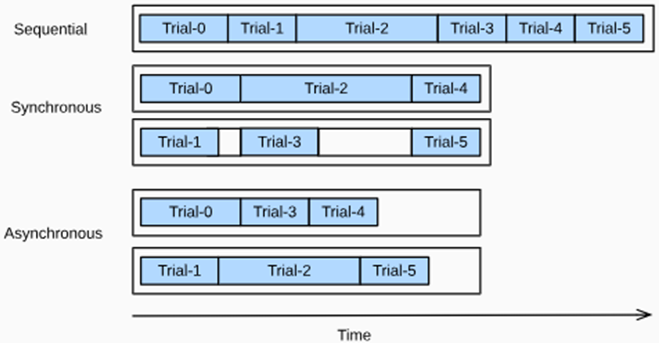
\includegraphics[width=12cm]{figures/figure-2.4.1.png}
	\caption[Comparsion of Sequential, Synchronous and Asynchronous Optimizations]{Comparsion of Sequential, Synchronous and Asynchronous Optimizations over time. Source:~\cite{Tesi-1.6}}
	\label{fig:figure-2.4.1}
\end{figure}

\myparagraph{Parallelization in Multi-Fidelity HPO:}
Pruning algorithms have to be parallelized just like Sampling algorithms.
\\[0.3cm]In Synchronous Pruning algorithms, a worker has to go through idle time in wait that all other workers on complete their subset of trials for the current Rung level. (Fig.~\ref{fig:figure-2.4.2})
\begin{figure}[t]
	\centering
	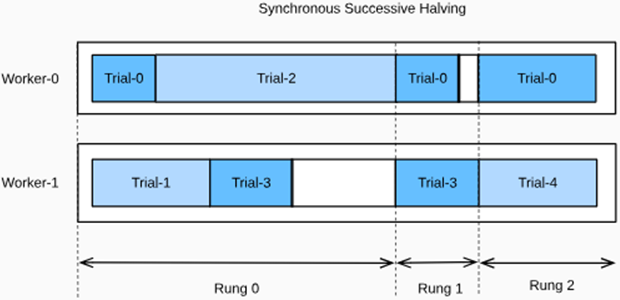
\includegraphics[width=12cm]{figures/figure-2.4.2.png}
	\caption[Functioning of Synchronous Optimization]{Functioning of Synchronous Optimization in Multi-Fidelity HPO techniques. Source:~\cite{Tesi-1.6}}
	\label{fig:figure-2.4.2}
\end{figure}
\\[0.3cm]In Asynchronous Pruning algorithms, a subset of configurations is promoted as soon as a specified number of observations are collected at the current Rung level. This may indeed lead to reduce the accuracy of promotions, but the impact on the final result is modest \cite{Tesi-1.6}. (Fig.~\ref{fig:figure-2.4.3})
\begin{figure}[t]
	\centering
	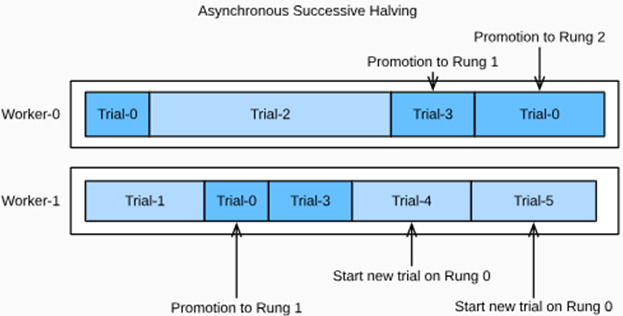
\includegraphics[width=12cm]{figures/figure-2.4.3.png}
	\caption[Functioning of Asynchronous Optimization]{Functioning of Asynchronous Optimization in Multi-Fidelity HPO techniques. Source:~\cite{Tesi-1.6}}
	\label{fig:figure-2.4.3}
\end{figure}

\subsection{Hyperparameters Overfitting}

When the Hyperparameter Optimization is completed, the chosen set of Hyperparameters are fitted on the training set and gets the best score.
The risk is that the model is overfitting. The Hyperparameter Optimization may overfit the hyperparameters values to the validation set.

\myparagraph{Solution to Possible Hyperparameters Overfitting:}
The solution is to evaluate the generalization performance (score) of the final model on a set that is completely independent to the one used to optimize the Hyperparameters.
This can be done with Nested Cross-Validation, a more complex Cross-Validation technique.
\\[0.3cm]In Nested Cross-Validation each fold in further divided into folds. The inner folds are used to tune the Hyperparameters, while the outer folds are used to evaluate the model’s performance as usual.

\subsection{Practical Aspects of HPO}

Some practical aspects of HPO.

\myparagraph{Choosing Evaluation Method:}
One often forgotten component of a HPO algorithm is the Evaluation method of the model or trial.
An ideal evaluator should be accurate, fast and simple. However, a trade-off remains between accuracy and speed; the more accurate, the probably more expensive it would be.
\\[0.3cm]The most used evaluation method is the traditional, that is, evaluation the current trial using the target Dataset, calculate its Accuracy (or other metrics).
Although this is by far the most precise method, it can be slow and resource wasting. Especially in DNNs tuning, where the number of configurations is very high, it is too expensive to evaluate traditionally each trial.
\\[0.3cm]Techniques like Early Stopping Strategies, which evaluate the model performance with an estimate function, rather than the actual evaluation function, allow to save time and resources during the evaluation process \cite{Tesi-1.8}.

\myparagraph{Choosing Performance Metrics:}
The choice of the Performance Metric to use for an Optimization Process, should derive from the real world context the model will work on.
In general, the most used metric is Accuracy, but in real world contexts it is a bad metric, and depending on the situation, Precision or Recall could be better; also F1-Score if both Precision and Recall are needed.
\\[0.3cm]Nevertheless, it remains true that for the most applications, it is impossible to determine a single metric able to capture all aspects of a model quality in a balanced manner \cite{Tesi-1.8}.

\myparagraph{Choosing the Search Space:}
Hyperparameters can be classified based on their domain of possible values.
Speaking of numeric HPs, there are mainly two different situations: Bounded in a closed interval (example: $[a,b]$); Bounded from below (example: $[0,\infty]$).
\\[0.3cm]HPs bounded from below can be tuned without modifications. HPs bounded in a closed interval need to be tuned on a logarithmic scale (example: $[\log a,\log b]$), in order to optimize performances.
\\[0.3cm]The size of the Search Space is also important. If the Search Space is too small, it may not contain well-performing Hyperparameter Configurations. If there are too many possible values for each HP, the cost of the search becomes too big. If there are too many HPs to tune, the algorithm will suffer from the Curse of Dimensionality.
Because of the problems coming from the size of the Search Space, it would be better to tune as few HPs as possible, each having as few possible values as possible \cite{Tesi-1.8}.

\myparagraph{Choosing the HPO Algorithm:}
The principal factor which determines which HPO algorithm to choose is the number of Hyperparameters.
\\[0.3cm]With a very small number of Hyperparameters, between 2 and 3, Grid Search could be the best option as it searches all the possible combinations; furthermore, is the easiest algorithm to interpretate and execute.
\\[0.3cm]As the number of HPs raises, between 3 and 10, Bayesian Optimization is the best option.
\\[0.3cm]If the number of HPs is very high, but the number of impactful HPs is low, then Random Search and Hyperband are the best choices.
\\[0.3cm]For Search Spaces which are both very large and complex, Evolutionary Algorithms and Iterative Racing are the best choices.
\\[0.3cm]One other factor that influences the algorithm choice is expensiveness of performance evaluation. If the evaluation process is expensive, then Multi-Fidelity algorithms like Hyperband are the best choices \cite{Tesi-1.8}.

\myparagraph{Choosing when to Terminate the HPO:}
There are different options for this problem.
\\[0.3cm]Option 1: defining an amount of runtime after which to stop the HPO, solely based on empirical data and intuition.
\\[0.3cm]Option 2: setting a lower bound regarding the generalization error. The problem with this solution is that the specified value could never be reached or could take the algorithm too much time to reach.
\\[0.3cm]Option 3: if no significant progress is made in a specified amount of time, the process is stopped. This option risks to stop the process too early.
\\[0.3cm]Option 4: (only for Bayesian Optimization and similar) when the acquisition function estimates that further progress is little or unlikely \cite{Tesi-1.8}.

\section{Hyperparameter Optimization Libraries}

Hyperparameter Optimization, as explained before, is an extremely computationally expensive operation, therefore each HPO algorithm needs to be the more optimized as possible.
Furthermore, HPO is a boring operation for the ML programmer, who seeks more automated approaches than Trial-and-Error and rerunning.
\\[0.3cm]For these reasons, libraries specifically designed to implement the HPO process exist.
Wrapping all HPO components and approaches in a single aimed library, allow to make the process the most optimized and organized as possible.

\subsection{Scikit-learn}

Scikit-Learn is a Python API for Machine Learning. It provides different algorithms for Hyperparameters Tuning \cite{scikit-learn}.
Scikit-Learn HPO algorithms versions are highly optimized and complete. Including parallelization, built-in resampling and OO approach.

\myparagraph{GridSearchCV and RandomSearchCV Classes:}
The simplest algorithm are Grid Search and Random Search, Scikit-Learn offer the two respective classes GridSearchCV and RandomSearchCV.
Both classes use Cross-Validation to evaluate the performance of the model, both classes require as input the model object of the tuning, and the Search Space, also called param\_grid.
\\[0.3cm]Other input parameters are: cv (number of folds for the Cross-Validation), scoring (the metric of evaluation used) and n\_jobs (number of CPU cores on which to parallelize the search).
\\[0.3cm]To start the Search for the best Hyperparameter combination, the fit() function must be called on the class object, passing as input X and y.
The fit() method has as output the object result, which contains the tuple of the best Hyperparameters and the score that particular tuple achieved.

\subsection{Optuna}

Optuna is a Python API for Machine Learning. In particular, the main functions Optuna provides concern Hyperparameter Optimization \cite{Optuna}.

\subsubsection{Introduction to Optuna}

Hyperparameter Optimization algorithms are often slow and poorly optimized. Moreover, these algorithms work better on some models and are bad on others.
Optuna is specifically designed to work with any Machine Learning or Deep Learning Framework \cite{Tesi-1.5}.

\myparagraph{Adavantages of Optuna:}
Optune combines all the good practices for the quality and the efficiency of Hyperparameter Optimization.
The search for the optimal Hyperparameters, for the best Hyperparameters combination is automated.
Searching and Pruning are automated and use the most efficient algorithms. This allows to obtain the best efficiency.
The parallelization process is easy and inexpensive, the search is run on multiple threads and multiple CPUs.

\subsubsection{HPO in Optuna}

Differently from most traditional approaches to Hyperparameter Tuning, Optuna divides the process in rigorous and ordered procedures.

\myparagraph{Workflow of Optuna:}
The workflow for the use of Optuna, is divided into 3 phases:
\begin{enumerate}[itemsep=0.1cm]
	\item Defining the Objective Function
	\item Creating a Study Object
	\item Running the Optimization Process
\end{enumerate}

\myparagraph{Optuna Phase 1 - Defining the Objective Function:}
The first big difference compared to traditional Hyperparameter Optimization is that the Search Space is not created from examples but is based on Suggestions.
\\[0.3cm]The Objective Function takes as an input a Trial object, on this object they can be called the suggest\_categorical() and suggest\_float() functions, respectively to generate suggestions (values) for Discrete and Continuous Hyperparameters.
(There are also other suggestions like: suggest\_int(), suggest\_loguniform(), suggest\_discrete\_uniform(), suggest\_uniform(). Each of which can take as input the low and high limits and the step).
\\[0.3cm]Inside the Objective Function, there are not only defined the Hyperparameters, but there is also the code for the definition, training, and evaluation of the ML model object of the tuning.

\myparagraph{Optuna Phase 2 - Creating a Study Object:}
The study object is created via the create\_study() function, which also defines the direction of the optimization (which depends on the evaluation criteria chosen).
\\[0.3cm]For Classification's evaluation metrics, the direction has to be “maximize”, for Regression's evaluation metrics, the direction has to be “minimize”.

\myparagraph{Optuna Phase 3 - Running the Optimization Process:}
The Optimization Process runs start form the study object, using the method optimize().
The method takes in input the Objective Function and the number of Trials.
\\[0.3cm]The method gives as output the number of the best trial, the accuracy of the best trial, and the tuple of Hyperparameters which represented the best trial.

\subsubsection{Samplers in Optuna}

In the field of study of Hyperparameter Optimization, Samplers define the way to sample the Hyperparameter values. Basically, the Samplers are the Search Algorithms.
The create\_study() function can take as input a Sampler, which will then be used as the search algorithm in the optimization process.
Optuna offers different Samplers.

\myparagraph{Tree-Structured Parzen Estimator (TPE) Sampler (TPESampler):}
Tree-Structured Parzen Estimator (TPE) Sampler is the default Sampler that Optuna uses. 
It is a particular case of Bayesian Optimization technique \cite{OptunaSamplers-TreeStructuredParzenEstimator}.

\myparagraph{Random Sampler (RandomSampler):}
Random Sampler samples Hyperparameters values randomly. It is equivalent to Random Search \cite{OptunaSamplers-RandomSearch}.

\myparagraph{Grid Sampler (GridSampler):}
Grid Sampler search across all different Hyperparameters in the Search Space. It is equivalent to Grid Search.

\myparagraph{CMA-ES Based Algorithm (CmaEsSampler):}
CMA-ES Based Algorithm (Covariance Matrix Adaptation Evolution Strategy) is a powerful search algorithm for continuous Search Spaces \cite{OptunaSamplers-CMA-ES}.

\myparagraph{Partial Fixed Sampler (PartialFixedSampler):}
Partial Fixed Sampler fixes the values of some Hyperparameters while optimizing the others. It is useful to explore the effects of single Hyperparameters or single smaller groups of Hyperparameters.

\myparagraph{Nondominated Sorting Genetic Algorithm II Sampler (NSGAIISampler):}
Nondominated Sorting Genetic Algorithm II Sampler is used to optimize multiple objectives simultaneously \cite{OptunaSamplers-NSGAII}.

\myparagraph{Quasi Monte Carlo Sampling Algorithm (QMCSampler):}
Quasi Monte Carlo Sampling Algorithm is a less randomic version of the Random Search. Provides better coverage of the Search Space compared to Random Sampling \cite{OptunaSamplers-RandomSearch}.

\subsubsection{Pruners in Optuna}

In the field of study of Hyperparameter Optimization, Pruners define the way to determine if and when to stop unpromising trials early.
Pruners allow to reduce the amount of time and resources used for the optimization process. Are used especially in situations where the dataset is very large, or the model is very complex.
\\[0.3cm]The create\_study() function can take as input a Pruner, which will then be used to valuate when to stop early a trial.
\\[0.3cm]Optuna offers different Pruners. (Although SuccessiveHalvingPruner and HyperbandPruner outperforms all the other, and are thus the only actually useful ones)

\myparagraph{MedianPruner:}
MedianPruner is based on the Median Pruning algorithm.

\myparagraph{NopPruner:}
NopPruner is based on the Non-Pruning algorithm.

\myparagraph{PatientPruner:}
PatientPruner is a Pruning algorithm with tolerance.

\myparagraph{PercentilePruner:}
PercentilePruner is a Pruning algorithm where the specified percentage of trials pass.

\myparagraph{SuccessiveHalvingPruner:}
SuccessiveHalvingPruner is based on the Asynchronous Successive Halving algorithm \cite{OptunaPruners-SuccessiveHalvingAlgorithm} \cite{OptunaPruners-AsynchronousSuccessiveHalvingAlgorithm}.

\myparagraph{HyperbandPruner:}
HyperbandPruner is based on the Hyperband algorithm \cite{OptunaPruners-Hyperband}.

\myparagraph{ThresholdPruner:}
ThresholdPruner is based on the Threshold algorithm.

\subsubsection{Other Aspects of Optuna}

Optuna is a big and powerful library, therefore offers a lot of specific functionalities.

\myparagraph{Callbacks in Optuna:}
Optuna allows to use Callback functions during the Optimization Process.
The defined Callback functions define a behaviour, an action, to execute at the end of each trial.
One common example of a callback function in this situation is a print function that prints some information regarding the current trial.

\myparagraph{Saving and Resuming Optimization Sessions in Optuna:}
Optuna allows to save permanently the results of an optimization, to interrupt an optimization session to resume it later, and even to share an optimization session across different machines.
All of this is done through the use of an SQLite Database, on which to store the data related to an optimization session.

\myparagraph{Feature Selection in Optuna:}
Optuna can be used in combination with apposite functions of Machine Learning libraries such as Scikit-learn to perform Feature Selection on the model in question.
Using the Optuna's suggestion functions, is possible to also tune the function for the Feature Selection.

\myparagraph{Visualizing Optimization Results in Optuna:}
Optuna preserves inside the study object some metadata that can be use to plot the history of the Optimization Process.
Through the module Visualization, Optuna offers different functions to plot different aspects of the Optimization Process.
\newline It can be plotted the History of the Optimization Process. (Fig.~\ref{fig:figure-2.5.1})
\begin{figure}[t]
	\centering
	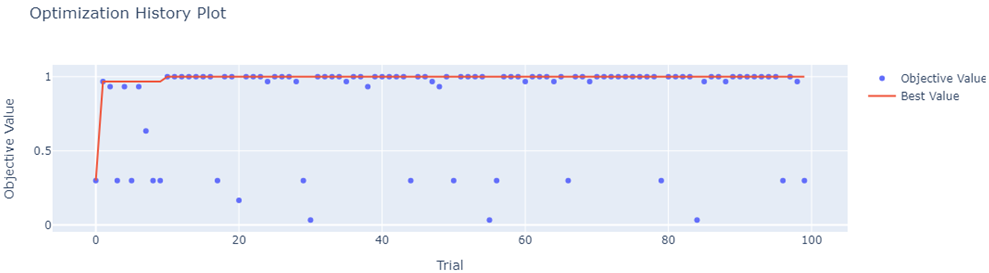
\includegraphics[width=16cm]{figures/figure-2.5.1.png}
	\caption[Optuna Optimization History Plot]{Optuna Optimization History Plot}
	\label{fig:figure-2.5.1}
\end{figure}
\newline It can be plotted the importance of some Hyperparameters over others. (Fig.~\ref{fig:figure-2.5.2})
\begin{figure}[t]
	\centering
	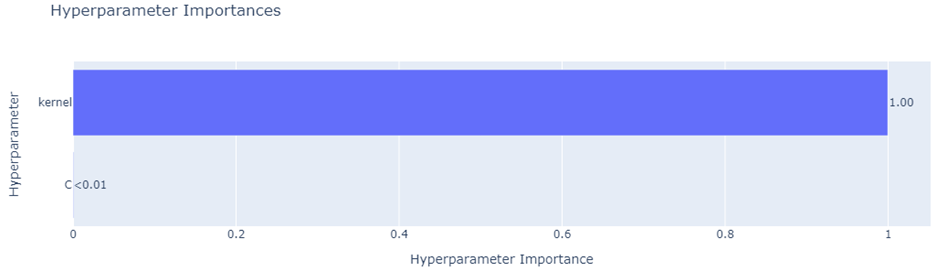
\includegraphics[width=16cm]{figures/figure-2.5.2.png}
	\caption[Optuna Hyperparameters Importance]{Optuna Hyperparameters Importance Plot}
	\label{fig:figure-2.5.2}
\end{figure}
\newline It can be plotted the relationship between Hyperparameters. (Fig.~\ref{fig:figure-2.5.3})
\begin{figure}[t]
	\centering
	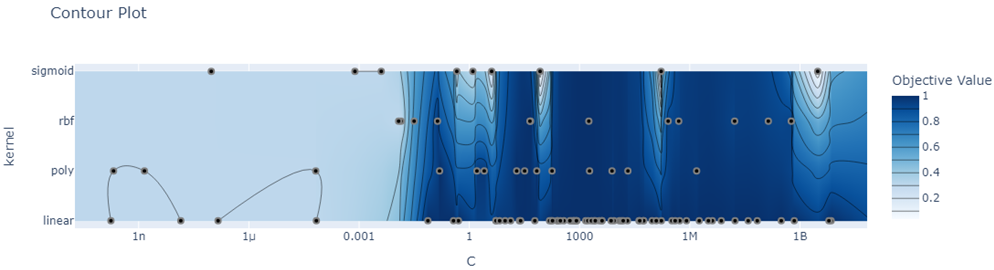
\includegraphics[width=15cm]{figures/figure-2.5.3.png}
	\caption[Optuna Contour Plot]{Optuna Contour Plot}
	\label{fig:figure-2.5.3}
\end{figure}
\newline It can be plotted the distribution of the trial result for each Hyperparameter value. (Fig.~\ref{fig:figure-2.5.4})
\begin{figure}[t]
	\centering
	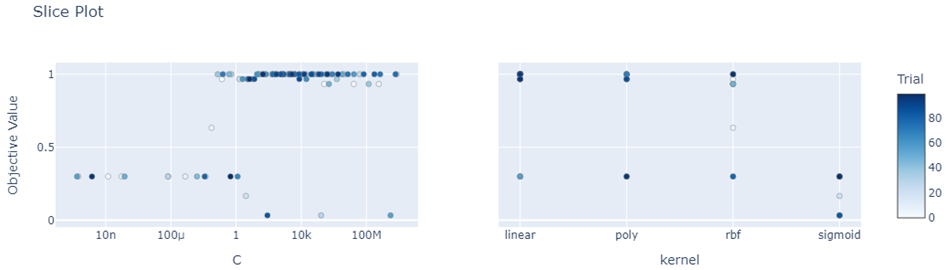
\includegraphics[width=15cm]{figures/figure-2.5.4.png}
	\caption[Optuna Trial Distribution Plot]{Optuna Trial Distribution Plot}
	\label{fig:figure-2.5.4}
\end{figure}
\\[2.5cm]

\section{Hyperparameter Optimization for Neural Networks}

HPO is a very computationally expensive process, which cost progressively increments as the Search Space, and so the number of HPs considered enlarges \cite{Tesi-1.9}.
Neural Networks, especially Deep Neural Networks, are the most complex type of ML model, and the number of HPs in a DNN model is very high.

\subsection{Main Hyperparameters for Neural Networks}

Therefore, an important aspect of HPO is understanding which of the Hyperparameters have the stronger effects on Parameters (in the case of NNs, Weights) during the training.
\\[0.3cm]Hyperparameters, especially when talking about Neural Networks, can be divided into two categories: Hyperparameters for Training, and Hyperparameter for model design.
\\[0.3cm]In Neural Networks, the most used Training related Hyperparameters are: Learning Rate, Batch-size, Activation Function, Optimizer (algorithm to update the weights, e.g. Gradient Descent, Adam). (Table~\ref{tab:table-2.6.1})
\\[0.3cm]In Neural Networks, the most used Model-Design related Hyperparameters are: Number of Hidden Layers, Width of Layers. (Table~\ref{tab:table-2.6.1})
\begin{table}[ht!]
	\center
	\setlength{\tabcolsep}{0.5cm}
	\caption[Common Hyperparameters in Neural Networks]{Table showing the most common Hyperparameters in Neural Networks and their suggested ranges of values.}
	\begin{tabular}{c c c c}
	Name & Type & Hyperparameter Range & log-scale\\[0.1cm]
	\hline\\[0.1cm]
	learning rate & float & $[10^{-6}, 10^{-1}]$ & yes\\[0.2cm]
	batch size & integer & $[8, 256]$ & yes\\[0.2cm]
	momentum & float & $[0, 0.99]$ & no\\[0.2cm]
	activation function & categorical & $\{$relu, sigmoid, tanh$\}$ & -\\[0.2cm]
	number of units & integer & $[16, 1024]$ & yes\\[0.2cm]
	number of layers & integer & $[1, 6]$ & no\\[0.2cm]
	\end{tabular}
	\label{tab:table-2.6.1}
\end{table}

\myparagraph{Learning Rate:}
Learning Rate is an Hyperparameter which determines the length of a “Learning Step”, it basically represents the velocity of learning.
The optimal value for the Learning Rate is different for every kind of problem, so in general only a few possibilities, one for each order of magnitude, are considered.
\\[0.3cm]More complex algorithms, use techniques such as Learning Rate Decay, where the value of Learning Rate decreases over time during the training, additional Hyperparameters are also introduced to tune this sub-algorithm \cite{Tesi-1.9}.

\myparagraph{Optimizer:}
Optimizer is the Hyperparameter which represents the algorithm used to update the Weights of the Neural Network.
More specifically is that algorithm which is used to minimize the Loss Function during the training, calculating the gradients of the loss function.
\\[0.3cm]The traditional Optimizer is Stochastic Gradient Descent; but nowadays there multiple more complex and better performing Optimizers, such as: Adam, RMSprop, Adagrad, Adadelta.
Most complex Optimizers have their own Hyperparameters, which optimal values choice depends on the type of the model and its other Hyperparameters.
\\[0.3cm]The choice of the Optimizer principally depends on the other HPs values. In general, Adam is well performing in most cases, RMSprop is good for Deep Networks \cite{Tesi-1.9}.

\myparagraph{Model Design Related Hyperparameters:}
The two most important HPs of this category for Neural Networks are Number of Hidden Layers, Width of Layers (or Number of Neurons in each Layer).
\\[0.3cm]The Number of Hidden Layers, generally speaking, grants the best accuracy results when it is a big number. Of course, this is a trade-off because the more Hidden Layers there are, the less lightweight the model will become, and so the more expensive it will become to train and tune.
\\[0.3cm]The Number of Neurons in each Layer, if it is too small will cause the model to underfit, if it is too big the model will overfit, and the cost of training would be too high. So, some suggestion can be followed: \cite{Tesi-1.9}
\begin{equation}
	w_{input} < w < w_{output}
\end{equation}
\begin{equation}
	w = \frac{2}{3} w_{input} + w_{output}
\end{equation}
\begin{equation}
	w < 2 w_{output}
\end{equation}

\myparagraph{Regularization:}
Regularization is a Hyperparameters which represents the Regularization function, that is, a function used to mitigate the model's overfitting and reduce the Generalization error.
\\[0.3cm]In general, the two most used Regularization techniques are L1 and L2, which both have their pros and cons, with L2 being the most used one. Although widely used for most ML models, for Neural Networks there are better alternatives.
\\[0.3cm]Data Augmentation add fake synthetic data to the training Dataset, in order to enhance the generalization power of the model.
\\[0.3cm]Dropout is the most used Regularization technique for NNs; during the training some Weights are “nulled”, simplifying the model and making it less likely to Overfit the training set, improving the generalization power \cite{Tesi-1.9}.

\myparagraph{Activation Function:}
Activation Function is a Hyperparameter which represents the mathematical function applied to the output of each Neuron.
The goal of Activation Function is to introduce non-linearity into the network, without which the model could not learn complex patterns.
\\[0.3cm]The most famous Activation Functions are the following: Sigmoid, Hyperbolic Tangent (tanh), ReLU, Softmax.
Sigmoid works well for simple Neural Networks, is less efficient for more complex models.
Softmax is only used in the output layer of NNs for Multiclass Classification.
\\[0.3cm]The most used Activation Function nowadays is ReLU, convient especially for its simplicity. Many variants of ReLU have being developed in the recent years such as Leaky ReLU, PReLU, ElU, SeLU.
Alternatives to ReLU are Maxout and Swish, which while they do resolve some problems of ReLU, are not that good for every situation \cite{Tesi-1.9}.

\subsection{HPO Algorithms applied to Neural Networks}

An overview on potential of each Major HPO algorithms category and their applicability for DNNs.
\\[0.3cm]A brief summary of the most important HPO algorithms, with advantages, disadvantages and applicability for Neural Networks, is showed in the following table. (Fig.~\ref{fig:figure-2.6.1})
\begin{figure}[t]
	\centering
	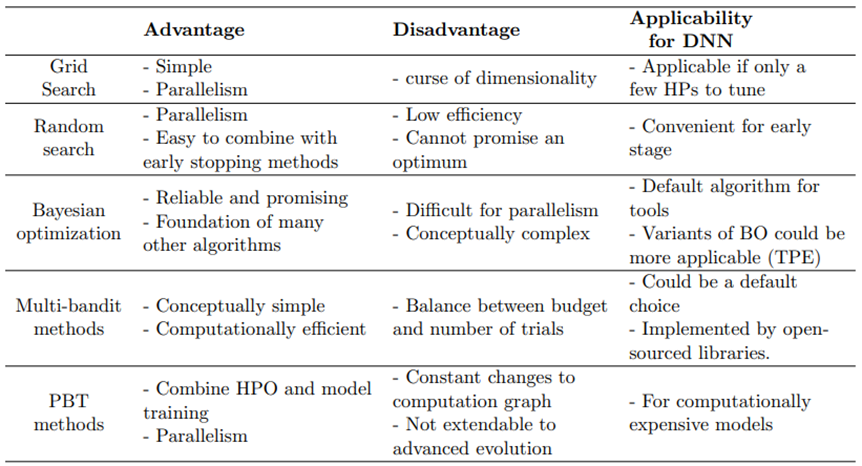
\includegraphics[width=15cm]{figures/figure-2.6.1.png}
	\caption[HPO Algorithm for NNs Summary]{Summary of main Hyperparameter Optimization Algorithms and their applicability to Neural Networks. Source:~\cite{Tesi-1.9}}
	\label{fig:figure-2.6.1}
\end{figure}

\myparagraph{Applicability to Deep Neural Networks:}
Grid Search is applicable only when a just a small subset of the DNN's HPs is searched. Moreover, the user needs to already have knowledge about empirical good values of the selected HPs to further narrow the search.
\\[0.3cm]Random Search can be used, only if combined with Early Stopping techniques, for the early stages of HPO.
\\[0.3cm]Bayesian Optimization, at least in its original form, is not ideal for DNNs tuning. Variants like TPE (Tree-Structured Parzen Estimator), which introduce parallelization, are appliable to many DNNs models.
\\[0.3cm]Multi-Armed Bandit algorithms (SHA, Hyperband, ASHA) are the default choice for DNNs' tuning. They outperform most algorithms in DNNs' models.
\\[0.3cm]Population Based Techniques are a good choice for large models and large datasets \cite{Tesi-1.9}.